\partopening{Price-Level Volatility Signals}{part:signals}
{Proposed daily and intraday methods, their calibration, and what they do on real prices.}

\section{The signal and the background variance}\label{sec:signaldesign}
The empirical target is a positive dependence of return variance on the
stock's price level after accounting for background volatility. The
motivation comes from a constant-elasticity diffusion
$\mathrm{d}S=\kappa S^p\mathrm{d}W$. Its instantaneous log-return variance is
$\kappa^2 S^{2(p-1)}$. We therefore use the convention
\begin{equation}\label{eq:betaconvention}
 \beta=2(p-1)
\end{equation}
throughout this manuscript. A positive $\beta$ is the direction associated
with strictness in that global, time-homogeneous diffusion. On observed
records it supplies a local statistical signature whose strength can be
estimated and compared across stocks and periods.

Background volatility is the main difficulty. A stock can rise during a
market-wide volatility expansion without its variance depending structurally
on its own price. Conversely, a state fitted flexibly to that stock's own
recent returns may absorb a genuine level effect. Our proposed methods make
different choices about which variation belongs to the background and which
remains available to identify the level signature.

\subsection{One conditional-return model on both sides}
Let $R_t=\log(S_t/S_{t-1})$ and let $x_{t-1}$ be log price relative to a
declared anchor. Write
\begin{equation}\label{eq:sharedmodel}
 R_t=\mu+\sqrt{v_t(\beta)}\,Z_t,
 \qquad v_t(\beta)=A_t\exp(\beta x_{t-1}),
\end{equation}
where $Z_t$ has a Student-$t$ law scaled to variance one and degrees of
freedom $\nu>2$. The same location, background-scale rule, and innovation
family enter both sides. The contrast is between $\beta>0$ and
$\beta\leq0$; including negative values allows variance to increase as the
price falls.

This conditional-return model is fitted under the observation law.
Stochastic-volatility processes provide separate stress cases for its
interpretation and calibration.

Let $\ell_n(\beta)$ be the accumulated log density over a scored record,
with nuisance quantities fixed or updated by their predeclared rule. A batch
contrast is
\begin{equation}\label{eq:batch}
 A_n^{\mathrm{batch}}=\sup_{\beta\geq0}\ell_n(\beta)
                         -\sup_{\beta\leq0}\ell_n(\beta).
\end{equation}
The implementation maps it to $\frac2\pi\arctan\max(0,A_n^{\mathrm{batch}})$.
This bounded score has many ties at zero, denoting no positive evidence
under the fitted contrast.

For monitoring, an equal-weight mixture over
$\mathcal B=\{1/8,1/4,1/2,1,2,4,8,16\}$ supplies the numerator:
\begin{equation}\label{eq:monitor}
 L_n=\log\left(\frac18\sum_{b\in\mathcal B}e^{\ell_n(b)}\right)
                    -\sup_{\beta\leq0}\ell_n(\beta).
\end{equation}
The mixture's predictive weights evolve using previous returns. The null
fits one common exponent to the whole prefix; it is not a product of
separately maximized one-step likelihoods. Reference records are scored over
their full scheduled horizons, and the reference distribution of the path
maximum sets the alarm cutoff.

Both profiles are numerical searches. Failures and unresolved profiles have
explicit statuses, are retained in denominators, and do not create positive
evidence. The real-data implementation is an empirically calibrated
statistic, not a certified sequential e-value. Appendix~\ref{app:algorithms}
gives the density, parameter domains, numerical conventions, and their
relationship to the separate exact-model guarantees.

\subsection{Daily market-scale construction}\label{sec:dailyconstruction}
For daily observations, anchor $x_{t-1}=\log(S_{t-1}/S_0)$ at the close
immediately preceding a launch. Use the last 20 completed SPY returns to form
\begin{equation}\label{eq:marketscale}
 M_t=\frac1{20}\sum_{j=1}^{20}(R^{\mathrm{SPY}}_{t-j})^2,
 \qquad m_t=M_t/M_{\mathrm{ref}},
 \qquad A_t=w m_t^g.
\end{equation}
Here $M_{\mathrm{ref}}$ is the geometric mean of the scale over the prior
252-session training period, frozen at launch. The background market scale
advances using completed market sessions. There is no stock-specific moving
variance recursion inside the scored window.

Fit $(\mu,w,g,\nu)$ under $\beta=0$ on the training returns, then freeze
them and score the following 252 returns. The batch statistic and the daily
monitor have separate calibrations. The stock's training data estimate the constant nuisance parameters; the
moving background state comes from SPY. A stock in SPY contributes to
its own proxy, with that dependence most direct when scoring SPY itself.

This construction asks whether positive own-level dependence remains after
one predictable market-scale adjustment. Independent stock-specific
volatility remains a source of residual variation, examined explicitly in
the simulations.
\source{experiments 055--056 and the D37 statistic design}

\subsection{Intraday session-anchor construction}\label{sec:intradayconstruction}
The intraday method uses regular-session five-minute closes. At each monthly
launch it estimates a diurnal clock from the preceding 252 sessions and
fits $(\mu,h_{\mathrm{init}},\nu)$ at $\beta=0$. Let $c_j$ denote the clock
for slot $j$, normalized to mean one. Within session $d$, use
\begin{equation}\label{eq:intradayscale}
 v_{d,j}(\beta)=h_d c_j
       \exp\!\left(\beta\log\frac{S_{d,j-1}}{s_d}\right),
\end{equation}
where $s_d$ is the session's first bar close. The state $h_d$ remains fixed
inside the session. After a completed session it updates from the mean
clock-adjusted squared residual, with a fixed 20-session half-life. The state
rule and fitted nuisance parameters are common to every exponent.

The level anchor resets each session while the likelihood evidence
accumulates across 21 sessions. A full launch has 1,617 adjacent five-minute
returns. Overnight returns are excluded. Missing required observations end
the supported prefix; early closes follow the declared schedule. This method
preserves within-session dependence that a variance state updating at every
bar could absorb. It can still absorb slower effects between sessions, and
the state can be misspecified during abrupt changes.

The original intraday implementation stores the exponent of standard
deviation, half the variance exponent used here. Its support
$\{1/16,\ldots,8\}$ is therefore the same as $\mathcal B$ in
\eqref{eq:monitor}. This notation change does not alter the algorithm.
\source{experiment 054; experiments 052--053 for its diagnostic motivation}

\subsection{Why the earlier likelihood score was replaced}
An earlier split-likelihood procedure selected an exact diffusion forecast
from a training catalogue and divided its likelihood by a drift- and
scale-profiled Gaussian null. It had an honest in-model guarantee, but its
real-data silence was not a clean demonstration of a fundamental power
barrier. In 2,287 of 3,000 broad-universe diagnostic windows, the forecast was
itself a null member, so the ratio could not exceed one. A training-selected
scale from a three-point grid also competed against a scale fitted on the
evaluation record. Scale misfit dominated the negative score in the cases
examined.

The diagnosis also found weak average daily separation even when fitting
on the evaluation record. A free-exponent likelihood contrast exceeded
$\log 20$ on 12.1\% of consensus positives and 11.7\% of calm controls.
Monthly realized-variance regressions controlling for market variance gave
pooled level elasticities of $+0.05$ (SE $0.04$) on run-ups and $+0.02$
(SE $0.08$) on consensus positives, compared with $-0.27$ on unselected
windows and $+0.59$ on calm controls. The construction problem and the weak
average signature were both part of the diagnosis.

The subsequent designs therefore changed how they isolate the pattern.
A shared Student-$t$ model repaired the likelihood comparison; the daily
market scale and intraday session anchor then preserved variation that an
own-stock volatility state could absorb. The resulting signals have
measurable simulation sensitivity and distinctive historical behavior,
reported below.
\source{experiments 049--051 for the diagnosis and initial repair;
054--056 for the later constructions}

\section{Calibration is part of the method}\label{sec:calibration}
A score ranks records according to a particular contrast. A threshold turns
that ranking into an operational decision. Two procedures can produce
similar rankings and very different alarm frequencies because their
reference distributions differ. Conversely, forcing both to flag 5\% of one
reference sample does not establish that they make the same errors on the
next population.

\subsection{The strict rank rule and its premise}
For $m$ reference scores $Z_1,\ldots,Z_m$ and target score $Z_*$, let
\begin{equation}\label{eq:rank}
 k=\lceil(m+1)(1-\alpha)\rceil,\qquad q=Z_{(k)},
 \qquad \text{alarm if }Z_*>q,
\end{equation}
with $q=+\infty$ when $k>m$. Under exchangeability of the selected references
and target, this rule has marginal rejection probability at most $\alpha$.
Strict exceedance preserves conservatism in the presence of ties. For
$m=499$ and $\alpha=0.05$, the cutoff is the 475th ordered reference score.
An additional zero floor can only reduce rejection.

This is a standard rank-calibration argument, applied to the entire score
construction \cite{tibshirani2019conformal}. For the monitor, the score used in
calibration is a complete record's maximum, so the controlled event concerns
at least one crossing during that declared horizon. It does not concern
indefinite monitoring, every monthly relaunch, or all stocks jointly.

The difficult premise is the score law \emph{after selection}. Choosing
references solely from the past prevents a form of look-ahead but does not
make calm references exchangeable with all future targets. Fitting nuisance
parameters, excluding missing records, choosing a market proxy, and changing
window lengths are all part of that law. Claim 045 supplies conditional
extensions with explicit distributional-error budgets, but those budgets
have not been estimated for the market replays here. Past-only selection is insufficient (claim 045), as is stationarity alone
(the separate counterexample in the refuted-research record).
\source{claim 045; \path{claims/refuted/d34-stationarity-calibration.txt}}

\subsection{A measured calibration effect on GSADF}
The lab first calibrated GSADF using 15 daily calm windows (103 name-records)
and 14 hourly calm windows (98 name-records). Each statistic was converted
to a simulated-random-walk p-value at the record's length. Empirical
thresholds were chosen from the calm records. Each calm window was then
evaluated against a threshold fitted on the other windows; positive episode
records used the threshold from all calm records.

\begin{table}[htbp]\centering\small
\begin{tabularx}{\linewidth}{@{}Yrrrr@{}}\toprule
Records & Conventional & Held-out calm & 95\% interval & Episodes\\
\midrule
\tablerows{generated/calibration.tex}
\bottomrule\end{tabularx}
\caption{GSADF flag rates (\%) at a 5\% reference target, before and after
empirical calibration. ``Conventional'' is the calm-record rate under the
simulated-null cutoff. ``Episodes'' uses the empirical cutoff. Intervals
resample whole calm windows; they are not independent-trial intervals.
Source: experiment 040.}\label{tab:gsadfcal}
\end{table}

Calibration substantially reduces calm-record flags while retaining many
episode flags: the daily full-record calm rate falls from 21.4\% to
6.8\%, with 63.6\% of episode records still flagged. The historical
experiment used interpolated quantiles and a tie-inclusive p-value rule,
not precisely \eqref{eq:rank}; later methods use the conservative rank rule.
The daily to-peak comparison uses an outcome-selected endpoint; the
full-record comparison avoids that particular selection.

Applying the daily cutoff unchanged to the broad universe reveals another
dimension. At 13-, 24-, and 72-month lengths, conventional GSADF flag rates
of 15.3\%, 19.0\%, and 33.2\% become 8.2\%, 10.9\%, and 23.0\%. In
2009--19, the corresponding calibrated rates are 6.4\%, 7.4\%, and 14.8\%.
A threshold fitted to shorter calm records does not transfer evenly to
six-year windows, even after converting the statistic to a random-walk
p-value. These are rates on unlabelled records, not estimates of size.
\source{experiments 039, 040, and 045; 416,380 overlapping name-windows}

\subsection{Exact-model guarantees and empirical calibration}
The research contains exact-model e-values as well as the empirical scores.
For a normalized forecast density $q$ and a null likelihood envelope
$\sup_{\theta\in\Theta_0}p_\theta$, the split-likelihood ratio is an e-value
when the true null density is included and the forecast is properly
conditioned on training information. This is an application of universal
inference \cite{wasserman2019universal}. e-BH can then control false
discoveries across names under arbitrary dependence
\cite{wang2020false}. Appendix~\ref{app:proofs} gives the argument.

The distinction is especially consequential for monitoring. Predictable
forecasts with a coherent whole-record null and certified likelihood bounds
support the lab's anytime-valid construction. The real-data Student-$t$
monitors instead freeze estimated nuisance parameters and use floating-point
profiles; the stated exact null premise and numerical certification are not
available. Their evidence is calibrated empirically as a statistic.

Known approaches to explosive-root testing already address changing
volatility, including time transformation
\cite{kurozumi2021time}. The lab's empirical calibration of GSADF is one
benchmark implementation. The comparisons below are against that
implementation, rather than the full family of volatility-robust tests.

\section{Simulation: recovery, power, and confounding}\label{sec:simulation}
The daily statistic has substantial sensitivity to positive level dependence
in its intended family. In the shared-market-scale and constant-volatility
CEV alternatives, its batch detection rate is 38.6--72.2\%, against
7.4--13.8\% for calibrated GSADF. These comparisons use matching null
calibrations and the same paths. They measure sensitivity to the specified
level alternatives; the methods' native null hypotheses differ.

\subsection{The daily market-scale method in its intended family}
The daily validation used 20 market warm-up sessions, 252 training sessions,
and 252 scored sessions. Each null cell had 499 calibration and 500
evaluation paths; each alternative had 500 evaluation paths. Methods used
the same generated observations. The fitted procedure was compared with
known nuisance parameters where defined, with its market exponent fixed to
zero, and with calibrated GSADF. Alternative cutoffs came from the matching
zero-level-effect family.

\begin{table}[htbp]\centering\small
\begin{tabularx}{\linewidth}{@{}Yrrrr@{}}\toprule
Generating model & Batch & Monitor & No-market batch & GSADF\\
\midrule
\tablerows{generated/simulation.tex}
\bottomrule\end{tabularx}
\caption{Selected simulation flag rates (\%) under matched calibration.
SV denotes stochastic volatility. The shared-market rows include both
innovation choices, $\nu=6$ and $10$; the persistent row has the effect in
training and scoring. GSADF is a
different-target comparator. Source: experiment 055.}\label{tab:sim}
\end{table}

The daily statistic recovers a known exponent in its own family. All
estimates in the six main recovery cells are finite; median relative errors
are at most 6\%. Eleven of twelve fitted/oracle recovery checks pass. The
failure is the fitted persistent-$\beta=1$ cell: 79.2\% of estimates are
positive against a declared 80\% target, while the known-nuisance version
passes. Absorption of a pre-existing level effect by the $\beta=0$ prior fit
is a plausible explanation for that shortfall.

Across 22 null cells, matched rates average 4.85\% for the fitted batch
statistic and 4.61\% for the monitor. Four exploratory per-cell checks fail
across the fitted, oracle, and no-market variants, and an extreme-negative-
exponent stress cell is unresolved because of numerical failures. These
rates describe the realized calibration cutoffs.

The power gains are substantive in the intended family. Using the market
scale instead of setting $g=0$ improves sensitivity in market-driven cells.
It adds little when the stock's volatility evolves independently of that
market. At $p=2$ with own-stock stochastic volatility, monitor sensitivity
is only about 10--20\% across the correlations tested. An external scale
helps when it tracks the nuisance variation actually present.

\subsection{What a positive fitted exponent can mean}
In the own-stock stochastic-volatility simulations, a structural
$\beta=0$ with positive price--volatility-driver correlation produces a
median fitted exponent of $+2.54$; negative correlation produces $-2.58$.
There is no true level term in either case. The statistic thus responds to
correlated stochastic volatility as well as to explicit local-level
dependence. This broader response is relevant to the positive-feedback mechanism in
Sin's model (Section~\ref{sec:sin}). It also means that the fitted exponent
measures an association shared by several mechanisms. The square-root
variance process used here is different from Sin's multiplicative factor;
its correlation response is evidence about the statistic, not a direct
application of Sin's strictness theorem.

The intraday estimator validation reaches a similar conclusion. With a
known level effect and independent volatility shocks, the within-day
estimator recovers its sign and approximate size. With structural
$\beta=0$ and driver correlation $-0.7$, its median is about $-4.1$.
Estimators using the stock's own smooth state attenuate a simulated positive
effect more than the within-day estimator. Together these experiments explain what the session anchor preserves: a
within-day price--variance association that faster own-stock state updates
can attenuate.
\source{experiments 053 and 055}

\subsection{Calibration transport can dominate the result}
The same daily statistic behaves very differently when calibrated on a
different variance law. Figure~\ref{fig:transport} applies the cutoff from
the baseline shared-market, $\beta=0$ family to other cells with no
structural level term. With own-stock stochastic volatility and positive
correlation, the monitor flags about 70\%, despite being near 5\% when
calibrated on the matching family. Regime-switching controls similarly
produce large increases in the full validation.

\begin{figure}[htbp]\centering
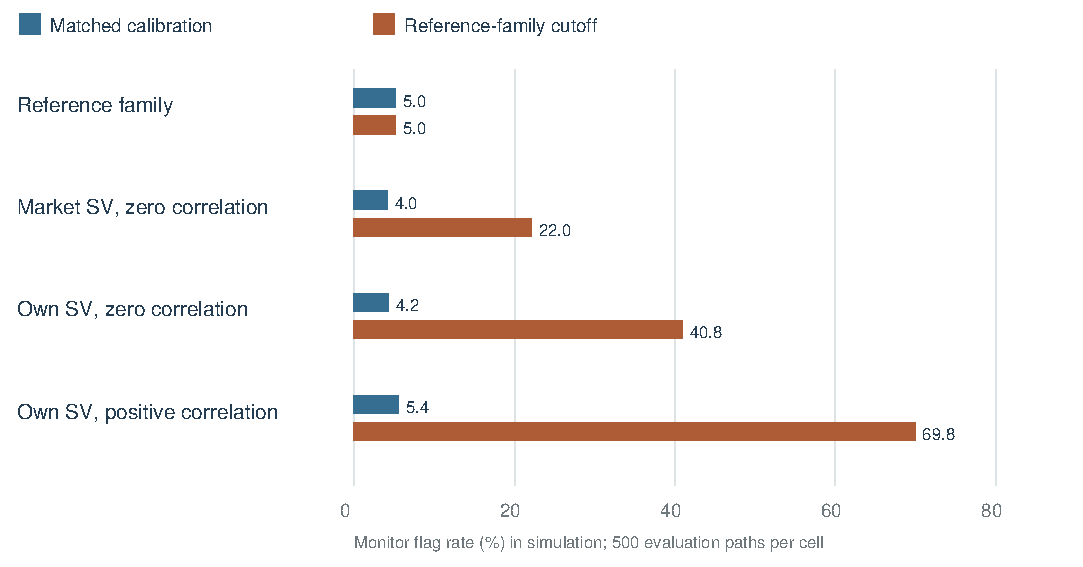
\includegraphics[width=\linewidth]{generated/calibration_transport.pdf}
\caption{The same daily monitor under matched and transported calibration.
``No level term'' is the structural simulation label; it does not claim
that all these models have the same pricing-martingale classification.
Source: experiment 055.}\label{fig:transport}
\end{figure}

This result explains why calibration is part of the method. Matched
calibration can absorb the distribution of a nuisance pattern, but the
price of doing so may be weaker separation from the alternatives. The relevant empirical question is how closely the reference library
resembles the target population in the features that drive the score.

The diffusion simulations were also compared at 10 and 50 substeps per day
using coupled increments. Fitted coefficients changed little; a later
check found four monitor alarm changes among 2,100 paired paths at fixed
coarse cutoffs, indicating relatively stable decisions at those resolutions.

\subsection{What the earlier exact-model experiments establish}
Exact constant-elasticity likelihoods offer a complementary benchmark. In a
two-exponent, four-scale catalogue, simulated null rejection was at most
0.1\% at a 5\% target. Against $p=2$, daily power rose from roughly
24--46\% over one year to 96--98\% over five years; five-minute sampling
gave nearly complete detection in the tested settings. This establishes
that level dependence can be statistically visible under strong model
restrictions.

Misspecification changes the picture. A geometric Brownian scale between
catalogue points was flagged 24\% of the time in a five-minute experiment.
Allowing a continuous Gaussian scale fixed that particular problem, but
repeated variance regimes broke the expanded procedure on daily panels.
Permitting switch dates restored validity within the switch model while
reducing power: in one five-year $p=1.5$ comparison, 44.7\% became 17.3\%
with a single admitted midpoint and 2.1\% when the middle 80\% of dates
were admitted. The experiment quantifies the sensitivity lost as that
particular comparison model becomes more flexible.

At high frequency, a declared intraday clock can preserve substantial
in-model power. Rounding and observation noise require their own
likelihood treatment. The lab's exact hidden-price filter avoids a
worst-case penalty at every rounded observation; certified calculations
were within roughly one log-likelihood unit of the ideal on simulated
\$5 geometric-Brownian null records of 30 and 125 days at cent ticks.
This is a result for that observation model, separate from the empirical
Student-$t$ replays.
\source{experiments 019, 022, 025--028; claims 033--038,
055, and 059. See the research map for the distinction between experiments
and formal results}

\section{Daily observations in the market}\label{sec:dailyresults}
The daily evidence has three roles: comparing historical episodes with calm
records; observing alarm behavior in a broader population; and checking
whether different constructions continue to differ after calibration.
Forecasting later outcomes is an additional exercise, considered after the
alarm results.

\subsection{Data and comparison design}
The early historical collection includes the dot-com period, financial and
housing-related names around 2007, and later run-ups. Separate records add
collapsed names where free data could be recovered. The broader study uses
the pinned current S\&P 500 constituents, with 416,380 overlapping windows
of 13, 24, or 72 months in the earlier analysis. It is unselected with
respect to the score, but not a historical point-in-time investment
universe.

Missing delisted names can change results in either direction. Failed firms
remove collapses; acquired firms can remove run-ups ending in takeover
premiums. The lab recovered only part of a union of public deletion lists,
with especially poor historical coverage before 2008. The direction of
survivorship bias is therefore ambiguous. Adjusted-close replays also use
a retrospective corporate-action record.

The daily market-scale replay uses monthly launches, 252 prior returns,
and a 252-session scored suffix. It starts in 1994 because SPY history and
the initial scale/training requirements constrain earlier dates. At each
launch, references are earlier completed universe records selected by a
calm-start predicate on training volatility and drawdown. Up to 499 are
taken in a fixed score-blind order, at most one per name per quarter.
The batch statistic, monitor maximum, and GSADF maximum receive separate
rank cutoffs from those same references.

\subsection{The daily market-scale signal changes the alarm pattern}
Among 150,519 universe launches with a finite calibration cutoff, the batch
statistic flags 2.91\%, the monitor 3.05\%, and GSADF 6.86\%. Including
3,197 early launches without a usable reference gives 153,716 launches and
the slightly lower rates used in Table~\ref{tab:daily}. Keeping these
denominators separate prevents the absence of a cutoff from appearing to
be successful non-rejection.

\begin{table}[htbp]\centering\small
\begin{tabularx}{\linewidth}{@{}Yrrrrr@{}}\toprule
Launch period & Launches & Batch & Monitor & GSADF & Calm batch\\
\midrule
\tablerows{generated/daily_periods.tex}
\bottomrule\end{tabularx}
\caption{Daily real-data flag rates (\%). ``Calm batch'' restricts to
calm-start records. Periods classify the launch, with the following year
scored. Early no-reference launches remain in this table. Source:
experiment 056.}\label{tab:daily}
\end{table}

\begin{figure}[htbp]\centering
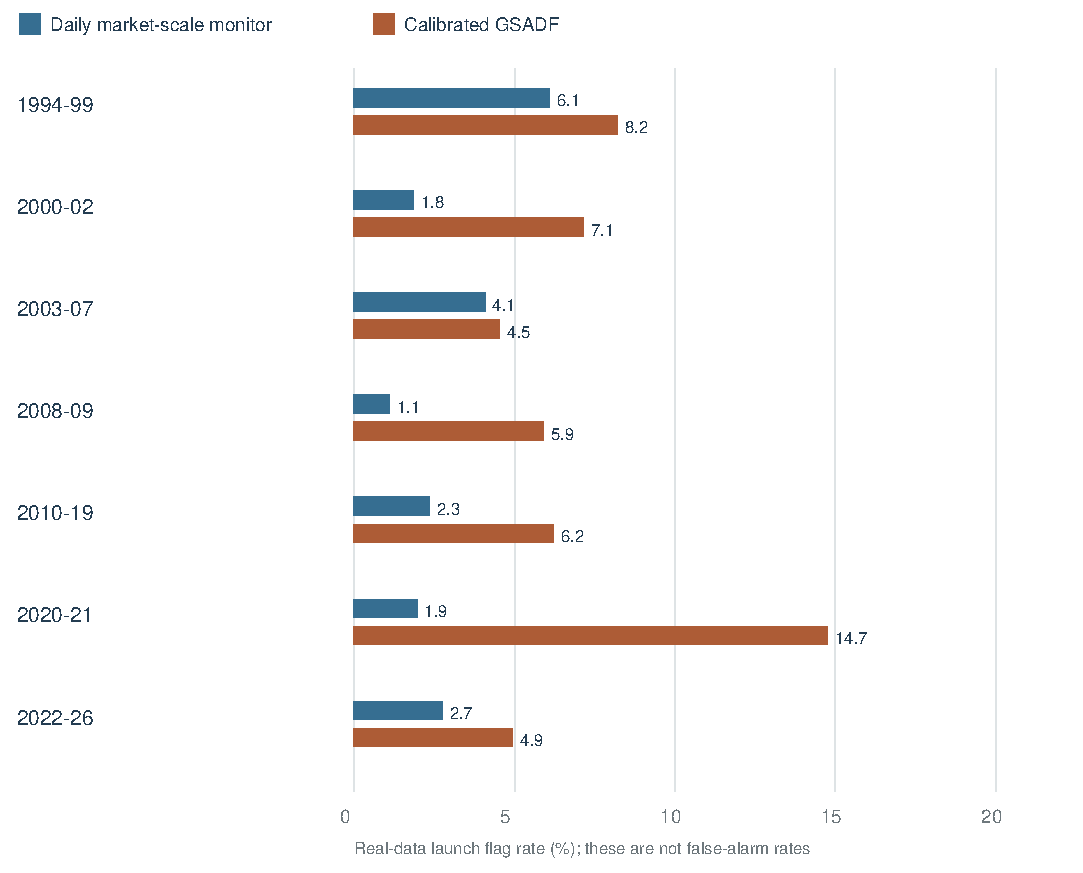
\includegraphics[width=0.95\linewidth]{generated/daily_flags.pdf}
\caption{Daily monitor and calibrated GSADF rates by launch cohort. Both
procedures use the same universe and earlier reference records. Source: experiment 056.}\label{fig:daily}
\end{figure}

The daily signal remains sparse in the three turbulent launch cohorts.
Batch rates are 1.8\% in 2000--02, 0.9\% in 2008--09, and 1.4\% in
2020--21; monitor rates are 1.8\%, 1.1\%, and 1.9\%. GSADF rates are
7.1\%, 5.9\%, and 14.7\%. The daily procedure's response therefore differs
substantially from an explosive-price screen, consistent with its design
of adjusting for common variance movements. The 1990s calm-start rate is
higher, so the contrast is specific to these cohorts.

\subsection{Homebuilders: a coherent early sector signal}\label{sec:homebuilders}
The four homebuilders provide the clearest daily case study. The monitor
flags D.R. Horton and Lennar in December 2003, then Pulte and Toll Brothers
in January 2004. Their respective price peaks occur in July 2005. All four
alarms precede the peaks by 377--411 trading sessions, a remarkably similar
lead across the sector. GSADF flags only Toll Brothers, 112 sessions before
its peak.

\begin{table}[htbp]\centering\small
\begin{tabularx}{\linewidth}{@{}Yllrr@{}}\toprule
Name & First daily alarm & Price peak & Daily lead & GSADF lead\\
\midrule
\tablerows{generated/homebuilders.tex}
\bottomrule\end{tabularx}
\caption{Homebuilder alarms in the registered 2003--08 records. Leads are
trading sessions before each record's price maximum; a dash denotes no
alarm. Source: experiment 056.}\label{tab:homebuilders}
\end{table}

This is evidence of a shared developing price--variance pattern well before
the sector's peak. For monitoring, identifying that development is a
useful distinct objective from predicting the date of reversal. The table
records first crossings; it does not measure the subsequent persistence or
intensification of the signal.

Across the wider collection, the daily monitor alarms before the peak on
15 of 30 supported consensus-positive records, against 14 for GSADF; on
the collapsed-name collection, the counts are 4 of 9 against 3. On 18 recent
narrative records, they are 7 against 10. The median pre-peak consensus lead
is 377 sessions versus 142 for GSADF. Results differ within financials:
BAC, JPM, AIG, and FNMA trigger after their peaks, while Lehman and
Countrywide trigger 107 and 833 sessions before theirs.

Two comparison conventions matter. Across consensus-negative records,
4.8\% of launches alarm and 35 of 91 records contain at least one alarm;
monthly relaunching creates more opportunities than a single launch.
GSADF also uses prior-inclusive history: 315 of its 650 alarmed episode
launches cross on the first scored day. These are comparisons of the
specified operational procedures.
\source{experiment 056, including its denominator and timing readings}

\subsection{How this differs from the repaired own-state score}
The earlier repaired daily score used a stock-specific volatility state.
On 10,000 universe windows, its empirical rate was 4.9\%, but yearly rates
ranged from about 1.4\% to 16.2\%. It flagged only 3 of the 33 requested
consensus positives, while flagging 20 of 103 calm controls; three non-US positive
records lacked complete histories on the imposed US calendar. Its consensus ranking had an AUC of 0.34,
with an interval containing 0.5. That repair had little episode discrimination under its specified design.

On common windows, the market-scale statistic has a rank correlation of
about 0.34 with that own-state score. Their distinct outputs show that changing the background-state treatment
materially changes the measurement.
\source{experiments 051 and 056}

\subsection{What the earlier alarms contain}
An audit of 185 flags from the earlier historical comparisons found that
156 survived a declared jump filter, including 137 of 153 explosive-root
flags. In daily records, rising volatility through the window was the
more distinctive feature: 69\% of flags exceeded the controls' 95th
percentile of the second-half/first-half volatility ratio. Removing jumps
increased the daily calm GSADF rate from 19.4\% to 25.2\%. This helps
explain why background variance and empirical calibration matter more than
simply deleting extreme returns in these comparisons.
\source{experiment 041; the audit concerns the earlier scores, not a new
jump-filter evaluation of the daily market-scale monitor}

\subsection{Implied volatility as a different background scale}
A separate construction used a lagged VIX or VXN value to scale a declared
Gaussian null. In simulation it had daily power against level dependence
not already reflected in that scale; dependence tracked by the supplied
scale was absorbed. In real SPX and NDX windows the registered scores were
silent, including the named historical episodes, apart from a few
crossings in a narrower sensitivity band. Some variance ratios fell outside
the declared band, and VIX before 22 September 2003 is a retrospective
backcast, making the earlier SPX windows reconstructed-scale analyses.
A separate stricter as-of design was withdrawn before scoring. The daily
market-scale method above uses a different background adjustment.
\source{claim 042; experiments 043 and 047}

\section{What five-minute data add}\label{sec:intradayresults}
The intraday evidence first examines the pattern, then evaluates the
specified monitor. These are different exercises: a coefficient estimated
on a whole retrospectively chosen episode is not an alarm available at its
beginning.

\subsection{Within-session variance behavior}
On the descriptive collection, the median within-day variance exponent is
$2.35$ for four meme-stock records and $1.48$ for 20 narrative-name
records. Four growth-name records have median $-3.59$; calm Dow members
have median $-5.94$. Most index estimates hit the lower search boundary
of $-20$, which is a numerical boundary, not an estimate beyond that
boundary. The meme records show positive fitted effects, while the growth
collection and some prominent narrative names show the usual negative
direction.

The pattern is less pronounced when one isolates hindsight-defined
run-up segments, and the estimates also respond to return--volatility
correlation in simulation. The empirical result is a difference in measured price--variance behavior
across these groups, encompassing both local-level and correlated-volatility
interpretations discussed in Section~\ref{sec:sin}.
\source{experiments 052--053; model-based curvature errors for the
within-day fits are distinct from empirical calibration}

\subsection{A retrospective replay of the monitor}
The specified monitor is calibrated on 499 calm-start references from
2017--18, all completed before targets begin in February 2019. It then
replays each 21-session launch with an assumed one-minute availability
delay. GSADF is evaluated at each daily close using the 252 prior closes
and the monitored sessions so far, with its own cutoff fitted to the
same reference IDs.

\begin{table}[htbp]\centering\small
\begin{tabularx}{\linewidth}{@{}Yrrr@{}}\toprule
Records & Launches & Intraday monitor & GSADF\\
\midrule
\tablerows{generated/intraday.tex}
\bottomrule\end{tabularx}
\caption{Launches with an alarm within the 21-session horizon (\%). The
run-up denominator retains training failures. The control rows reuse
name-launches across episode windows and are descriptive. Source:
experiment 054.}\label{tab:intraday}
\end{table}

The intraday monitor alarms on 46.2\% of meme-stock launches. Across all
run-up records the rate is 19.6\%. GSADF alarms
more often on these episodes and on none of the selected calm controls.
Of 29 run-up records, the monitor alarms strictly before the peak on 14,
GSADF on 20, with one additional GSADF alarm on the peak date. The
monitor's median pre-peak lead is 142 sessions, compared with 57.5 for
GSADF. Seven monitor alarms precede the defined run-up onset; only seven
fall between onset and peak.

There are important availability and timing differences. Of 449 run-up
launches, 109 fail before fitting because fewer than 200 prior sessions
have at least 70 bars. Seven records never obtain a successful launch.
The failures remain in the rates. GSADF uses the available daily history,
and 163 of its 182 alarmed positive launches cross on the first monitored
session. Thus the table compares procedures that can be deployed under
the declared rules, with GSADF benefiting from more daily history at launch.

The calm-control table has 1,127 weighted entries but only 610 distinct
name-launches. The monitor alarms on 30 of those distinct launches,
4.9\%; the weighting in the displayed table yields different subgroup
rates. Inference must account for repeated names and dates. In an
unselected 100-name draw, the monitor alarms on 5.0\% of 8,600 launches,
versus 5.4\% for GSADF, with its own annual rate varying from 2.3\% to
9.8\%. These frequencies describe the broad-draw population under the
fixed reference calibration.

The direct daily/intraday comparison also favors the faster observations
for early recognition. Among the 29 common run-up records, both monitors
alarm somewhere in 14, with the intraday alarm earlier in 13 of those.
Five records have only a daily alarm, six only an intraday alarm, and four
neither. Counting strictly pre-peak alarms, the totals are 13 daily and 14
intraday. These are the registered record definitions; three names have
different peak dates in the two source experiments.
\source{experiment 056, comparison with experiment 054}

\subsection{Incremental out-of-sample drawdown information}
The intraday score supplies the first positive incremental out-of-sample
drawdown result in this sequence of lab scores. Adding it to GSADF raises
predictive $R^2$ from 1.05\% to 1.39\% at 63 sessions and from 1.49\% to
1.74\% at 126 sessions. Thus the intraday statistic contains information
that the explosive-root score alone leaves out of these fitted forecasts.

Regressions use within-launch-date ranks, an intercept, and either or both
scores. Outcomes start after the completed scoring window. Coefficients
are trained on records whose outcomes end before 2023 and evaluated on
launches from 2023 onward.

\begin{table}[htbp]\centering
\begin{tabular}{@{}rrrr@{}}\toprule
Forward sessions & Intraday alone & GSADF alone & Combined\\
\midrule
\tablerows{generated/forecast.tex}
\bottomrule\end{tabular}
\caption{Out-of-sample $R^2$ (\%) for maximum drawdown, relative to the
training mean. The rows concern completed-window scores, not first
alarms. Source: experiment 054.}\label{tab:forecast}
\end{table}

The gains of 0.34 and 0.25 percentage points are point estimates; paired
uncertainty for the improvements was not computed. These score-only
regressions also leave open how much information survives controls for
realized volatility and momentum. This is the scope of the forecasting
finding, which is supplementary to the measurement and alarm results.
Neither score demonstrates return predictability in this exercise. The
daily market-scale score's drawdown $R^2$ is much smaller, approximately
0.03--0.16\%, with no demonstrated useful incremental gain over GSADF.

\section{Reading and using an alarm}\label{sec:use}
The proposed signals answer a conditional measurement question. An alarm
means that the fitted positive-level alternative accumulated unusually
large evidence relative to the declared comparison model and reference
records. It is useful to inspect the estimated level pattern, background
scale, data support, and the behavior of alternative calibrations together.
A large raw likelihood contrast with an unusual reference history is a
different finding from a stable contrast across several predeclared
reference choices.

The daily and intraday results suggest complementary descriptions. The
daily market-scale construction produces relatively sparse alarms and
has demonstrable model-based power when the market proxy tracks the
nuisance. The intraday construction detects within-session patterns in
some speculative episodes and adds out-of-sample drawdown information.
GSADF remains the stronger general episode alarm in the intraday
comparison. The new scores contribute different measurements: selective
daily patterns and an intraday component that improves the combined forecast.

For ongoing monitoring, two further results from the research matter.
First, repeatedly relaunching a monitor changes the error event. The
exact-model framework can fund declared or adaptive restarts from one
budget; it cannot discard unfavorable evidence and restart for free.
Second, dependence across names does not invalidate e-BH when genuine
e-values are supplied, but it does not make an empirical score an e-value.
Reviewer simulations of pooled forecasts found no improvement over per-name
alternatives. Experiment 029 likewise found essentially no detection gain
from selecting a cross-sectional clock within its specified model; outside
that model, selection could damage false-discovery control.

The construction of an exact filter for rounded prices is another useful
methodological result. It treats the hidden efficient price jointly across
the record instead of paying an independent worst-case penalty at each
observation. That result belongs to an exact observation model. Applying
it to recorded trade closes with different noise and rounding mechanisms
requires a new model check, not merely a finer sampling interval.

